\chapter{\ifenglish Background Knowledge and Theory\else ทฤษฎีที่เกี่ยวข้อง\fi}
\tolerance = 9999
\overfullrule=0pt

% การทำโครงงาน เริ่มต้นด้วยการศึกษาค้นคว้า ทฤษฎีที่เกี่ยวข้อง หรือ งานวิจัย/โครงงาน ที่เคยมีผู้นำเสนอไว้แล้ว ซึ่งเนื้อหาในบทนี้ก็จะเกี่ยวกับการอธิบายถึงสิ่งที่เกี่ยวข้องกับโครงงาน เพื่อให้ผู้อ่านเข้าใจเนื้อหาในบทถัดๆ ไปได้ง่ายขึ้น
\enskip \enskip \enskip ในการตรวจสอบประกาศนียบัตรออนไลน์ด้วยบล็อคเชนก่อนที่จะลงมือสร้างนั้นผู้พัฒนาจำเป็นที่จะต้องไปศึกษาเกี่ยวกับ Blockchain 
ก่อนสำหรับสร้างซึ่งจะไปศึกษาจาก Hyperledger Fabric และใช้ Blockchain แบบ private
โดยเนื้อหาในบทนี้จะอธิบายในส่วนของความรู้ ทฤษฎีบทที่เกี่ยวข้อง และหลักการต่างๆที่ผู้พัฒนาได้ศึกษา และนำไปใช้ในการสร้าง Blockchain  
เพื่อให้ผู้ที่เข้ามาอ่านได้เข้าใจหลักการต่างๆในเบื้องต้น และเพื่อให้เข้าใจเนื้อหาในบทถัดๆไปได้ง่ายมากยิ่งขึ้น

\section{พื้นฐาน Blockchain}
\enskip \enskip \enskip \enskip \enskip 
\enskip \enskip 
\subsection{Blockchain คืออะไร}
\cite{Blockchain}
Blockchain คือเทคโนโลยีว่าด้วยระบบการเก็บข้อมูล Data Structure ซึ่งไม่มีตัวกลาง แต่ข้อมูลที่ได้รับการปกป้องจะถูกแชร์และจัดเก็บเป็นสำเนาไว้ในเครื่องของทุกคนที่ใช้ฐานข้อมูลเดียวกันเสมือนห่วงโซ่ Chain โดยทุกคนจะรับทราบร่วมกัน ว่าใครเป็นเจ้าของและมีสิทธิในข้อมูลตัวจริง เมื่อมีการอัปเดตข้อมูลใด ๆ สำเนาข้อมูลในฐานเดียวกันก็จะอัปเดตตามไปด้วยทันที ทำให้การปลอมแปลงข้อมูลไม่ใช่เรื่องง่าย เพราะทุกคนต้องรับทราบและตรวจสอบความถูกต้องของข้อมูลร่วมกันได้ อีกทั้งไม่มีระบบล่ม และภัยใด ๆ ก็ไม่อาจทำลายอุปกรณ์ในระบบได้พร้อมกัน เช่นเดียวกับการถูกแฮ็กข้อมูล ซึ่งต้องทำการแฮ็กทุกเครื่องในฐานเดียวกันพร้อม ๆ กัน หรืออย่างน้อยต้องแฮ็กเครื่องที่ถือสำเนาให้ได้มากกว่าร้อยละ 51 จึงจะแฮ็กได้สำเร็จ เทคโนโลยี Blockchain จึงนับว่ายอดเยี่ยมในแง่ของเครดิตและความปลอดภัย นอกจากนี้ ยังเป็นเทคโนโลยีที่เข้ามารองรับการซื้อขายสกุลเงินดิจิทัล เช่น บิทคอยน์ Bitcoin ฯลฯ ให้มีความปลอดภัยด้านข้อมูลมากยิ่งขึ้นด้วย
\subsection{Blockchain แตกต่างจาก Database ทั่วๆไปอย่างไร}
\cite{Blockchain_a}
คือ Blockchain จะมีการเก็บข้อมูลไว้เป็นกลุ่มๆ ไว้ใน block ซึ่งมัดรวมข้อมูลไว้ด้วยกัน ซึ่งมีการเก็บข้อมูลจะในมาต่อกับ block ก่อนหน้ามีลักษณะเป็นโซ่ ซึ่งถ้าข้อมูลก่อนหน้าผิดพลาดหรือถูกแก้ไขจะทำให้รู้ได้เพราะเหมือนโซ่ที่ขาดออกจากกัน แต่ในส่วนของdatabase ทั่วๆไปจะเก็บในรูปแบบของตารางซึ่งถ้าถูกแก้ไขจะทำให้เราไม่รู้ตัวได้ว่าถูกแก้ไขเมื่่อใด แต่ถ้า Blockchain  
\subsection{Public blockchain คือ}
\cite{Blockchain_b}
คือ เป็น Blockchain ที่ทุกคนสามารถเข้าถึงและมีส่วนร่วมได้ เนื่องจากเป็น Open Network ทั้งหมด โดยลักษณะของการใช้งานพื้นฐานของ Blockchain ประเภทนี้ คือ การแลกเปลี่ยน Cryptocurrency และการขุด รวมถึงความสามารถในการรักษาความไว้วางใจระหว่าง Community ของผู้ใช้ทั้งหมด 
เนื่องจากทุกคนในเครือข่ายรู้สึกมีแรงจูงใจที่จะทำงานเพื่อพัฒนาเครือข่าย แต่ข้อเสียของ Blockchain ประเภทนี้ คือ ต้องใช้พลังงานจำนวนมากในการประมวลผลธุรกรรมเพราะใช้ระบบ Proof of work ในการตรวจสอบธุรกรรม และปัญหาอีกอย่างที่พบเจอคือ การเปิดกว้างเกินไป จึงทำให้ไม่มีความเป็นส่วนตัวในการทำธุรกรรมเท่าไรนัก
ตัวอย่างของ Public blockchain network เช่น Bitcoin  , Ethereum , BNB Chain ซึ่งต่างเป็น Blockchain ยอดนิยมที่ทุกคนสามารถเข้าถึงได้ง่าย
\subsection{Private blockchain คือ}
\cite{Blockchain_b}
คือ Blockchain ที่ทำงานในเครือข่ายแบบปิด ซึ่งสามารถเข้าร่วมได้เฉพาะบุคคลที่ได้รับอนุญาตหรือคำเชิญเท่านั้น โดย Blockchain ประเภทนี้เหมาะที่สุดสำหรับองค์กรและธุรกิจที่ต้องการใช้ Blockchain สำหรับการใช้งานภายใน 
ขณะที่การทำธุรกรรมใน Private blockchain นั้นเร็วและง่ายเมื่อเทียบกับ Public blockchain แต่ข้อเสีย คือ ไม่มีการกระจายอำนาจ เนื่องจากมีผู้มีอำนาจเพียงคนเดียวที่ดูแลเครือข่าย
\subsection{ข้อดีของ Blockchain}
\cite{Blockchain_a}
คือ ช่วยเพิ่มความปลอดภัยของข้อมูลและสามารถรู้ได้ว่าข้อมูลของเราถูกแก้ไขหรือดัดแปลงไหม

\section{พื้นฐาน Hyperledger Fabric}
\enskip \enskip \enskip \enskip \enskip
\cite{Hyperledger} 
Hyperledger Fabric เป็น private blockchain ซึ่งหมายความว่า ใครก็ตามที่ต้องการเข้าร่วมและใช้งานข้อมูลบน chain ในระบบ จะต้องได้รับสิทธิ์ก่อน จึงสามารถมองเห็นและใช้งานข้อมูลที่อยู่ใน chain นั้นๆได้ ซึ่งจะแตกต่างจาก public blockchain ที่ไม่ว่าจะเป็นใครก็สามารถมีสิทธิ์เข้าถึงข้อมูลบน ledger ได้นั่นเอง

Hyperledger Fabric เป็น Distributed Ledger ถูกออกแบบมาเพื่อใช้งานเกี่ยวกับการทำ transaction ระหว่างองค์กร โดยแต่ละองค์กรจะมีช่องทางที่ใช้สำหรับ communicate ซึ่งกันและกัน โดยที่องค์กรหนึ่งๆสามารถอยู่ได้หลายช่องทาง และแต่ละช่องทางนั้นข้อมูลจะถูกแยกจากกันอย่างชัดเจน

ด้วยพื้นฐานของโครงการที่ต้องการให้ Architecture ของ Hyperledger Fabric มีลักษณะเป็น Modular ตัว Hyperledger Fabric จึงประกอบด้วย Component สำคัญๆดังต่อไปนี้
\subsection{Peers}
\cite{Hyperledger_a} 
 โดยส่วนตัวหากจะให้จินตนาการว่า Peers คืออะไร ก็ให้นึกถึง Network แบบ Peer-to-Peer โดย Peer ในที่นี้ก็คือ Node แต่ละ Node ภายใต้ Network ของ Blockchain นั้นๆ นั่นเอง
 \graphicspath{ {./images/} }
 \begin{figure}[htbp]
   \centering 
   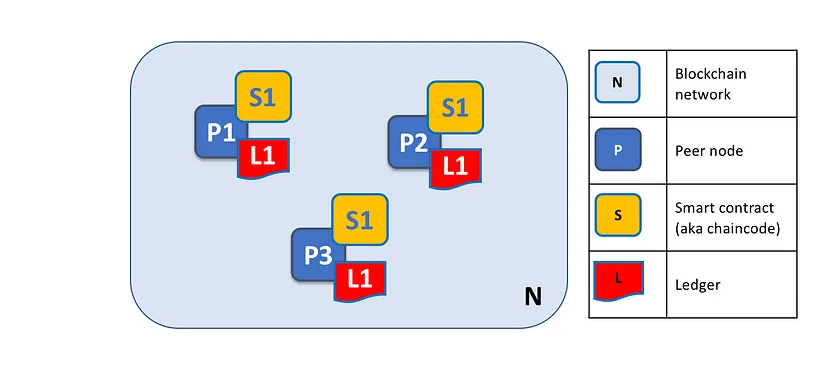
\includegraphics[scale=0.2]{peer.png}
   \caption[Peer]{ตัวอย่างของpeer
   ที่มา: https://hyperledger-fabric.readthedocs.io/en/release-2.2/peers/peers.html}
   \label{fig:Peer}
 \end{figure}



\subsection{Certificate Authorities}
\cite{Hyperledger_a} 
หากพูดถึง Blockchain ก็ต้องบอกว่ามันเป็นกลุ่มของ Network ที่ทำหน้าที่ประมวลผลข้อมูลร่วมกัน โดยเฉพาะใน Permissioned Blockchain อย่าง Hyperledger Fabric ที่เราจำเป็นต้องรู้ว่าคนที่เข้ามาเป็นใคร ตัวจริงหรือไม่ มีสิทธิ์ในการเข้าถึง Network ในรูปแบบใดบ้าง
\graphicspath{ {./images/} }
\begin{figure}[htbp]
  \centering 
  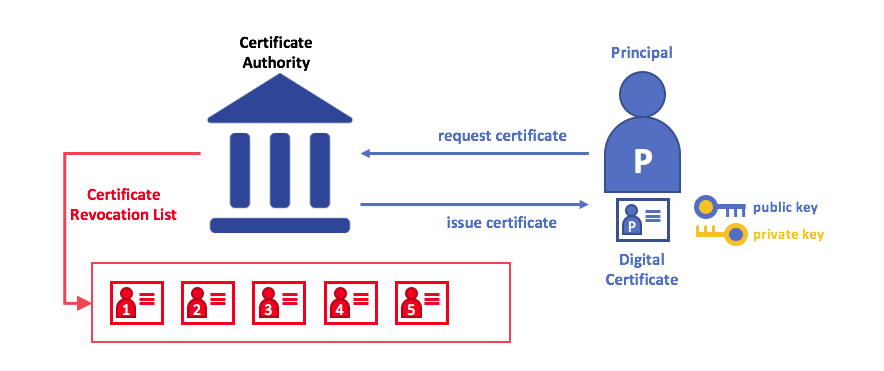
\includegraphics[scale=0.5]{certifi.png}
  \caption[Certificate Authorities]{Certificate Authorities
  ที่มา:https://hyperledger-fabric.readthedocs.io/en/release-2.2/peers/peers.html}
  \label{fig:Certificate}
\end{figure}

Certificate Authorities มีหน้าที่ Generate Identity ของทุกๆ Actor ที่ต้องการใช้งาน Network ของ Blockchain โดย Certificate Authorities จะสร้าง Digital Certificate ที่ระบุตัวตนของ Actor ตามมาตรฐาน X.509

\subsection{Ordering services}
\cite{Hyperledger_a} 
ในโลกของ Hyperledger Fabric Ordering Service จะทำหน้าที่หลักๆ 2 ส่วน คือ
\begin{enumerate}
  \item Pack ตัว Transaction ที่ต้องการแก้ไข Ledger ที่ส่งเข้ามาจาก Application แต่ละตัว 
  \item กระจาย Pack ของ Transactionที่สร้างขึ้นนั้น ไปยังแต่ละ Peer ที่อยู่ใน Network
\end{enumerate}

โดยในแต่ละ Transaction ของการจัดการกับข้อมูลที่อยู่ใน Ledger จะประกอบไปด้วย 3 ระยะ คือ

\begin{enumerate}
  \item Proposal
  เป็นระยะที่เกิดขึ้นหลังจากที่ Application ปลายทางส่ง Request เข้ายัง Endorser เพื่อสร้าง Proposal สำหรับ Update ข้อมูล ขั้นตอนนี้เสร็จสิ้น Endorser จะส่ง Response กลับไปที่ Application
  \item Proposal
  เป็นระยะที่เกิดขึ้นหลังจากที่ Application ปลายทางส่ง Request เข้ายัง Endorser เพื่อสร้าง Proposal สำหรับ Update ข้อมูล ขั้นตอนนี้เสร็จสิ้น Endorser จะส่ง Response กลับไปที่ Application
  \item Validation and commit
  เมื่อ Peers ได้รับข้อมูล Transaction จาก Ordering Services หากข้อมูลมีความถูกต้องก็จะ Commit เข้าไปใน Ledger ของตัวเอง
\end{enumerate}

\subsection{Channels}
\cite{Hyperledger_a} 
หากจะเปรียบเทียบว่า Channel ใน Hyperledger Fabric คืออะไร ก็ให้นึกถึงช่องทางที่เปิดให้เข้าถึงในแต่ละ Peer ของ Network นั้นๆ
\graphicspath{ {./images/} }
\begin{figure}[htbp]
  \centering 
  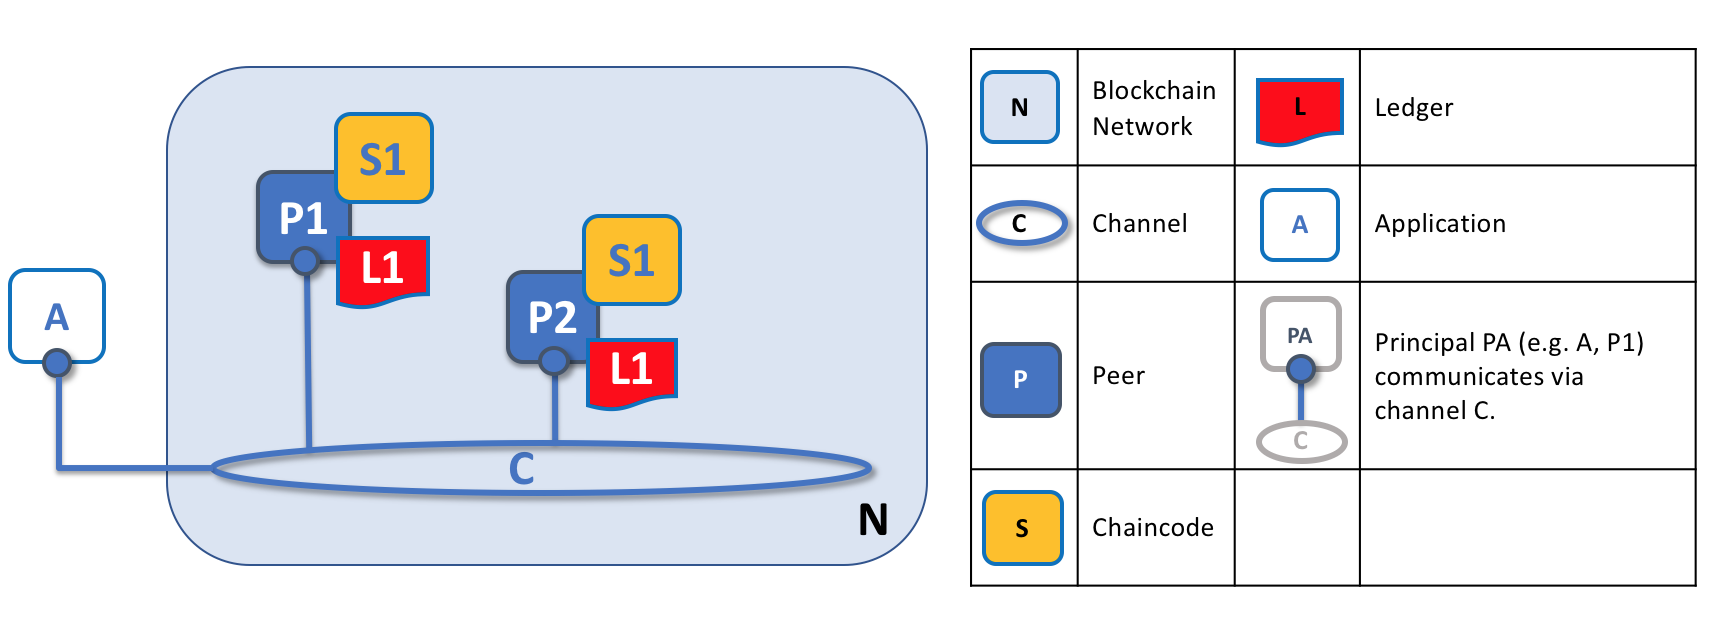
\includegraphics[scale=0.5]{peers diagram 5.png}
  \caption[Peers Diagram 5]{peers diagram 5
  ที่มา:https://hyperledger-fabric.readthedocs.io/en/release-2.2/peers/peers.html}
  \label{fig:peers diagram 5}
\end{figure}

ยกตัวอย่างในรูป การจะเข้าที่ Peer P1 และ P2 ได้ ก็จำเป็นที่จะต้องเข้าผ่าน Channel C ที่ถูกสร้างขึ้น แต่ถ้าหากใน Network นี้มี Peer P3 อยู่ในภายใน Network Application A ก็จะไม่สามารถเข้าถึงได้ เนื่องจาก Channel C ที่ถูกสร้างขึ้น ไม่ได้เชื่อมต่อกับ Peer P3 ที่ถูกสร้างขึ้นนั้นเอง

\subsection{Chaincode หรือ Smart Contracts}
\cite{Hyperledger_a} 
หากใครใช้งาน Eterium ก็คงจะรู้จัก Smart Contract ที่เขียนด้วย Solidity ของ Eterium มาบ้างเช่นกัน โดย Concept อาจจะไม่ต่างกัน โดย Chaincode จะมีลักษณะเหมือนโปรแกรมขนาดเล็ก ที่เปิดให้ Application ส่งคำสั่งเข้ามาประมวลผลข้อมูลที่อยู่ภายใน Ledger ได้ สำหรับ Hyperledger Fabric เปิดให้นักพัฒนาสามารถพัฒนา Chaincode ผ่านทาง Fabric SDK ได้ด้วยภาษาที่ค่อนข้างหลากหลาย ได้แก่ Go, Javascript หรือ Java

\section{\ifenglish%
\ifcpe CPE \else ISNE \fi knowledge used, applied, or integrated in this project
\else%
ความรู้ตามหลักสูตรซึ่งถูกนำมาใช้หรือบูรณาการในโครงงาน
\fi
}
\enskip \enskip \enskip \enskip \enskip ในการทำโครงงานนี้กลุ่มของพวกเราได้นำความรู้ตามหลักสูตรต่างๆ มาประยุกต์ใช้ ซึ่งได้แก่
\enskip \enskip \enskip \enskip \enskip 
\subsection{Database Systems (261342) }
ในการออกแบบdatabase เราจะใช้ความรู้ในการออกแบบการเก็บข้อมูลแบบ offchain ว่าออกแบบยังไงให้เก็บข้อมูลครบถ้วนและไม่มากเกินไป

\subsection{NET AND INFO SECURITY (261447) }
ใใช้ความรู้ในการออกแบบ Smart Contracts ว่าออกแบบยังไงให้ปลอดภัยไม่ถูกโจมตีและรับมือกับการโจมตีอย่างไรหรือทำให้สามารถรู้ตัวได้ไวว่าโดนโจมตี


% \begin{center}
% 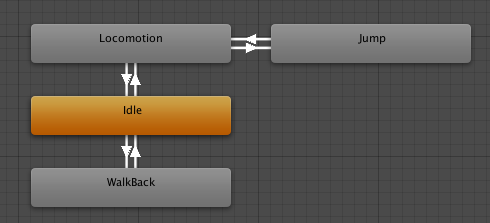
\includegraphics[scale=0.6]{MecanimStateMachine.png}
% \end{center}
% \begin{center}
% รูปที่ 2.2: ตัวอย่าง State Machine ที่ใช้ควบคุม animation
% \end{center}
% \graphicspath{ {./images/} }



% \subsubsection{Subsubsection 1 heading goes here}
% Subsubsection 1 text

% \subsubsection{Subsubsection 2 heading goes here}
% Subsubsection 2 text

% \section{Third section}
% Section 3 text. The dielectric constant\index{dielectric constant}
% at the air-metal interface determines
% the resonance shift\index{resonance shift} as absorption or capture occurs
% is shown in Equation~\eqref{eq:dielectric}:

% \begin{equation}\label{eq:dielectric}
% k_1=\frac{\omega}{c({1/\varepsilon_m + 1/\varepsilon_i})^{1/2}}=k_2=\frac{\omega
% \sin(\theta)\varepsilon_\mathit{air}^{1/2}}{c}
% \end{equation}

% \noindent
% where $\omega$ is the frequency of the plasmon, $c$ is the speed of
% light, $\varepsilon_m$ is the dielectric constant of the metal,
% $\varepsilon_i$ is the dielectric constant of neighboring insulator,
% and $\varepsilon_\mathit{air}$ is the dielectric constant of air.

% \section{About using figures in your report}

% define a command that produces some filler text, the lorem ipsum.
% \newcommand{\loremipsum}{
%   \textit{Lorem ipsum dolor sit amet, consectetur adipisicing elit, sed do
%   eiusmod tempor incididunt ut labore et dolore magna aliqua. Ut enim ad
%   minim veniam, quis nostrud exercitation ullamco laboris nisi ut
%   aliquip ex ea commodo consequat. Duis aute irure dolor in
%   reprehenderit in voluptate velit esse cillum dolore eu fugiat nulla
%   pariatur. Excepteur sint occaecat cupidatat non proident, sunt in
%   culpa qui officia deserunt mollit anim id est laborum.}\par}

% \begin{figure}
%   \centering

%   \fbox{
%      \parbox{.6\textwidth}{\loremipsum}
%   }

%   % To include an image in the figure, say myimage.pdf, you could use
%   % the following code. Look up the documentation for the package
%   % graphicx for more information.
%   % \includegraphics[width=\textwidth]{myimage}

%   \caption[Sample figure]{This figure is a sample containing \gls{lorem ipsum},
%   showing you how you can include figures and glossary in your report.
%   You can specify a shorter caption that will appear in the List of Figures.}
%   \label{fig:sample-figure}
% \end{figure}

% Using \verb.\label. and \verb.\ref. commands allows us to refer to
% figures easily. If we can refer to Figures
% \ref{fig:walrus} and \ref{fig:sample-figure} by name in the {\LaTeX}
% source code, then we will not need to update the code that refers to it
% even if the placement or ordering of the figures changes.

% \loremipsum\loremipsum

% % This code demonstrates how to get a landscape table or figure. It
% % uses the package lscape to turn everything but the page number into
% % landscape orientation. Everything should be included within an
% % \afterpage{ .... } to avoid causing a page break too early.
% \afterpage{
%   \begin{landscape}
%   \begin{table}
%     \caption{Sample landscape table}
%     \label{tab:sample-table}

%     \centering

%     \begin{tabular}{c||c|c}
%         Year & A & B \\
%         \hline\hline
%         1989 & 12 & 23 \\
%         1990 & 4 & 9 \\
%         1991 & 3 & 6 \\
%     \end{tabular}
%   \end{table}
%   \end{landscape}
% }

% \loremipsum\loremipsum\loremipsum

% \section{Overfull hbox}

% When the \verb.semifinal. option is passed to the \verb.cpecmu. document class,
% any line that is longer than the line width, i.e., an overfull hbox, will be
% highlighted with a black solid rule:
% \begin{center}
% \begin{minipage}{2em}
% juxtaposition
% \end{minipage}
% \end{center}





% อธิบายถึงความรู้ และแนวทางการนำความรู้ต่างๆ ที่ได้เรียนตามหลักสูตร ซึ่งถูกนำมาใช้ในโครงงาน

\section{\ifenglish%
Extracurricular knowledge used, applied, or integrated in this project
\else%
ความรู้นอกหลักสูตรซึ่งถูกนำมาใช้หรือบูรณาการในโครงงาน
\fi
}
\enskip \enskip \enskip \enskip \enskip ในการทำโครงงานนี้กลุ่มของพวกเราได้นำความรู้นอกหลักสูตรต่างๆ มาประยุกต์ใช้ ซึ่งได้แก่

\subsection{ความรู้ทางด้านการทำงานของ Blockchain}
\enskip \enskip \enskip เนื่องจากกลุ่มของเราไม่มีความรู้ด้าน Blockchain จึงต้องไปศึกษา Blockchain ดังที่กล่าวไว้ในข้อ 2.1 พื้นฐาน Blockchain ว่า Blockchain มีการทำงานอย่างไร

\subsection{ความรู้การใช้งาน Hyperledger Fabric}
\enskip \enskip \enskip เนื่องจากพวกเรามีการใช้ Blockchain แบบ Private Blockchain จึงเลือกใช้ Hyperledger Fabric  ในการพัฒนา กลุ่มของพวกเราจึงได้ทำการศึกษาเพิ่มเติมกันเอง
โดยอาศัยสื่อต่างๆทางอินเตอร์เน็ต เช่น youtube, google เป็นต้น ดังที่กล่าวไว้ในข้อ 2.2 พื้นฐาน Hyperledger Fabric


\subsection{ความรู้ทางด้านการใช้ docker}
\enskip \enskip \enskip เนื่องจากเราต้องใช้ docker ในการจำลองการเปิดเซิร์ฟเวอร์ในการส่งข้อมูลจากหลายๆที่เราจึงต้องไปศึกษาการใช้ dockerเบื้องต้น



% อธิบายถึงความรู้ต่างๆ ที่เรียนรู้ด้วยตนเอง และแนวทางการนำความรู้เหล่านั้นมาใช้ในโครงงาน
